\begin{anexosenv}

	\partanexos
	% \includepdf[pages=-,pagecommand=\chapter{Protocolo PKS}]{./anexanexospk/Protocolo_PKS.pdf}

	\chapter{Documento de Arquiteruta}
	\section{introdução}
	Esta documento descreve a arquitetura e tecnologias da aplicação, utilizadas no desenvolvido do sistema de auxilio na detecção da doença de Parkinson utilizando Tremor em repouso. Desenvolvido pelos alunos de Trabalho de Conclusão de Curso 2 da Universidade de Brasília.

	Será desenvolvida uma aplicação web, podendo facilmente ser migrada para uma aplicação mobile em projetos futuros.

	\section{Tecnologias}
	\subsection{Single Page Aplication - SPA}

	\subsection{REST}
	Baseado no baseado no protocolo de comunicação de rede HTTP, sendo simples, rápida e com uma fácil comunicação entre clientes e servidores. Funciona com objetos em formato JSON, e os métodos definidos no protocolo HTTP ( POST, GET, PUT e DELETE) possibilitando assim uma eficiente e rápida troca de informação.

	\section{Representação da Arquitetura}
	A arquitetura se baseia me dois modelos arquiteturais, REST e SPA, interligados com um modelo de aprendizado de máquinas, no caso o Randon Forest ou o SVM, como observado na figura A Figura \ref{diagramadepacotes}. Ou sejá possui três pacotes:

	\begin{itemize}
		\item Machine Learning models;
		\item API;
		\item Web.
	\end{itemize}

	\begin{figure}[!htb]
		\centering
		 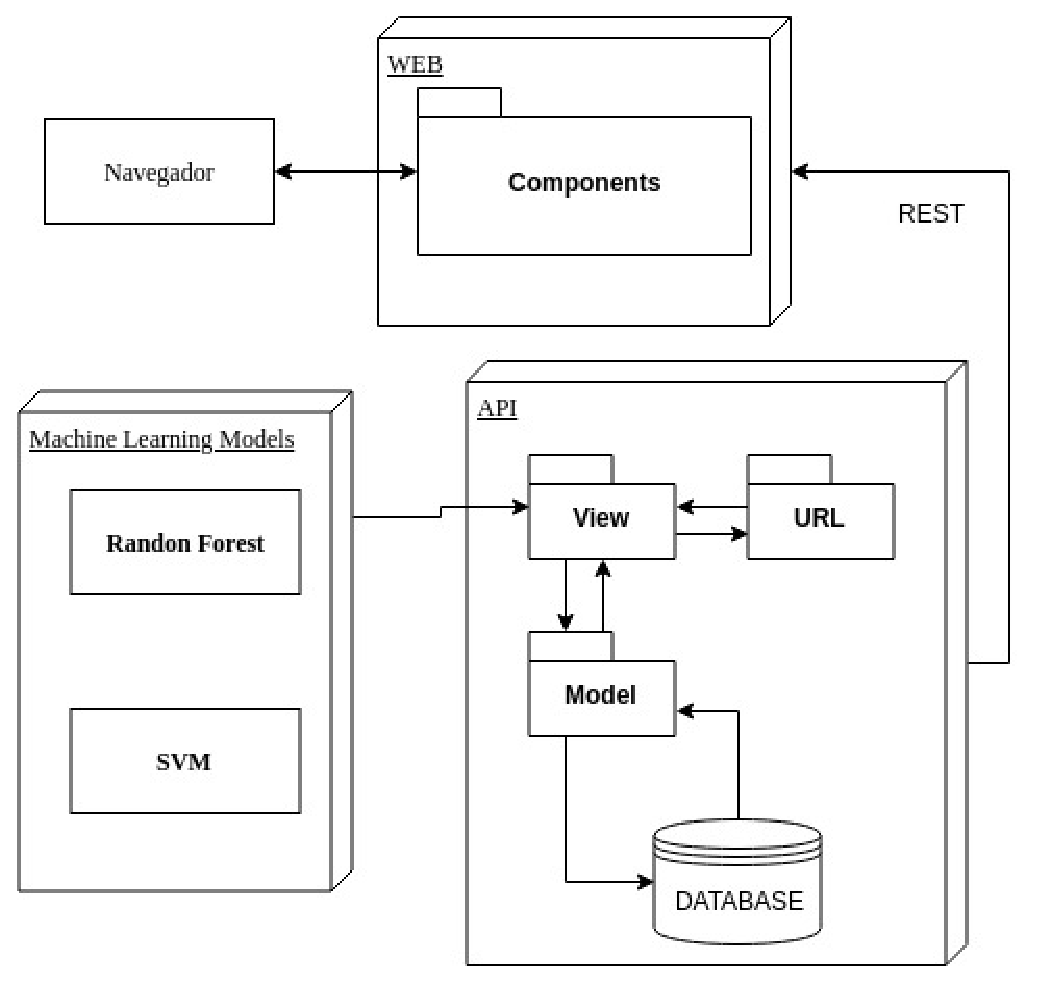
\includegraphics[width=0.9\textwidth]{figuras/diagrama_pacotes.eps}
		 \caption{Diagrama de pacotes}
		 \label{diagramadepacotes}
	 \end{figure}

	\subsection{Machine Learning models}
	Consiste no modelo já treinado e vallidado do algoritimo Randon Forest, sendo que este é armazenado no banco de dados \textit{PickleDB}. Deste modo, a comunicação é somente de leitura, com o modelo sendo enviado por completo para a API.
	\subsection{API}
	A API execulta todas as manipulações envolvendo os dados, como o pré-processamento do arquivo enviado pelo usuário, e classificando estes com o modelo salvo. Além de salvar os dados no banco de dados e envia-los quando requisitados, foi desenvolvida utilizadando os padrões de projeto definidos pelo Django-Rest-Framework, possuindo o mair esforço na \textit{View}.

	No caso as seguintes classes foram desenvolvidas, sendo elas:
	\begin{enumerate}
		\item InsertFeature: realiza o cadastro de um paciente.
		\item ListAllPatients: lista todos os pacientes, retornando-os em um objeto JSON.
		\item DetailPatient: retorna os detalhes relativos a um único paciente.
		\item UpdatePatient: possibilita a edição de um paciente já cadastrado.
		\item CLS: possui apenas um método GET, que recebe um id de um paciente. Com auxilio de outros métodos carrega o arquivo sEMG associado a este paciente, realiza o pré-processamento aplicando a FFT, carrega o modelo e por fim retorna o resultado da classificação.
	\end{enumerate}
	
	\subsection{Web}
	Responsável pela exibição dos dados, desenvolvido em react, possui somente três componentes, cadastrado, editar e home.
	
	\section{Restrições e Metas Arquiteturais}
	\section{Visão Lógica}
	\subsection{Diagrama de Classes}
	\subsection{Diagrama de Pacotes}
	\section{Referências}

\end{anexosenv}

